% Outline Project Specification Report

%The document is a report
\documentclass[12pt,a4paper]{article}

%define horizontal rule
\newcommand{\HRule}{\rule{\linewidth}{0.5mm}}

\usepackage{fullpage}
\usepackage{pdfpages}
%use the listings package
\usepackage{listings}
%use the English language
\usepackage[english]{babel}
%use graphics
\usepackage{graphicx}
%use wrap figures
\usepackage{wrapfig}
%geometry stuffs
\usepackage{lscape}
%use natbib bibliography package
%\usepackage[numbers]{natbib}
%use harvard bibliography package
%\usepackage{harvard}	
%use captions
\usepackage{caption}
%use multi-row tables
\usepackage{multirow}
\usepackage{url}
\usepackage{subcaption}


\usepackage[nottoc,numbib]{tocbibind}

\begin{document}

%use harvard citations
%\citationstyle{agsm}

%include the title page
\newcommand{\Revision}{678f948}

\begin{titlepage}
 
\begin{center}

% Upper part of the page

\includegraphics[width=0.20\textwidth]{../cover_logo.png}\\[1cm]


\textsc{\LARGE Aberystwyth University}\\[0.5cm]
\textsc{\LARGE Final Report}\\[0.5cm]



 
% Title
\HRule \\[0.4cm]
{ \huge \bfseries Partridge: An Intelligent Literature Analysis and
Recommendation Suite.}\\[0.4cm]

\HRule \\[1.5cm]

 % Author and student ID
\begin{minipage}{0.4\textwidth}
\begin{flushleft} \large
\emph{Author:}\\
\textsc{James Ravenscroft}\\
jrr9@aber.ac.uk\\
090407039\\
\end{flushleft}
\end{minipage}
\begin{minipage}{0.4\textwidth}
\begin{flushright} \large
\emph{Supervisors} \\
Amanda Clare (afc)\\
Maria Liakata (mal)

\end{flushright}
\end{minipage}


\vfill

\textsc{Submitted in partial fulfilment of requirements for a Batchelor of
Science Degree at Aberystwyth University}



\vfill
 
% Bottom of the page
\textsc{\large Word Count: 0}\\
\textsc{\large Status: Draft}\\
\textsc{\large Revision: \Revision{} }\\
{\large \today}
 
\end{center}

\frontmatter
 
\end{titlepage}



%some definitions for paragraph layout stuff
\setlength{\parindent}{0pt}
\setlength{\parskip}{1.5ex plus 0.5ex minus 0.2ex}

\tableofcontents

\pagebreak

\section{Project Summary}

This document describes the creation of Partridge, a new web-based tool
designed to assist in information processing and knowledge acquisition within
the domain of scientific research.

Since the advent of the 'Digital Age' and the ability of computers to copy and
reproduce information for a negligible cost, the amount of information
available to researchers has been increasing drastically.  B-C Bj\"{o}rk (2009)
estimates that approximately 1.4 Million papers were published in the year 2006
alone\cite{bjork2009}. Moreover, the growing popularity of Open Access
publishing (making papers available to readers for free online\cite{Suber2012}) across
most scientific disciplines\cite{bjork2009}\cite{harnad2004comparing} is
providing scientists and researchers with an even larger volume of information to be
processed. As available information increases, relevant material becomes
progressively more difficult to find and the need for an automated information
retrieval tool more apparent. The problem is even more vital for General
Practitioners. Goldacre (2008:97) points out that ``there have been an
estimated 15 million medical academic articles published so far, and 5000
journals published every month... picking out what's relevant is a gargantuan
task."\cite{goldacre2008bad} 

Partridge's main objective is to provide reading recommendations and
information retrieval for scientists and researchers. This should reduce the
amount of extraneous information that users have to read for themselves by
helping them find information specific to their interests more quickly.
Partridge will achieve this through the use of several existing techniques in
Natural Language Processing which are discussed below.

From the point of view of it's users, Partridge will assist researchers in two
ways. The system will provide filtering of papers based upon their
specific domain (i.e. is the paper primarily concerned with methodology within
an experiment in chemistry or is it about ethics in psychological studies?) and
their result, whether the paper yielded positive, negative or inconclusive
evidence for a hypothesis. Depending upon the time constraints of the
project, it is hoped that Partridge will also offer a user 'profiling' system
that provides recommendations for researchers based on their reading history.
This feature should help users find relevant papers more quickly or find
research that they may have otherwise overlooked.

Search engines such as Google ({\url{http://www.google.com/}}), and social
citation management tools such as CiteULike ({\url{http://www.citeulike.org}}),
do offer some assistance in tracking down relevant information. However, these
tools are often too general or rely upon the user knowing exactly what keywords
to use before carrying out the search. These drawbacks are further discussed in 
Section \ref{sec:prior_art} below.

To overcome the drawbacks of these existing systems, Partridge will make use of
several cutting edge Artificial Intelligence (AI) techniques in order to analyse and
process the papers in a more in depth way. AI is a very complex and field and
implementing the above features will be incredibly challenging. To help with
this, Partridge will build upon the system implemented by Liakata et al. for
recognising hypotheses, methods, results, conclusions and a number of other
scientific concepts in scientific articles \cite{citeulike:10444769}. The
Natural Language Toolkit for Python will also be used to build models for
recognising different fields and topics, classifying results as positive or
negative and recognising different types of papers, from case studies to
methodology papers\cite{bird2009natural}.

\section{Current Progress}

\subsection{Background}

\subsubsection{Artificial Intelligence}
In science fiction literature and films, Artificial Intelligence (AI) and the
ability of machines to automatically process and understand human language is
almost always taken for granted. The current state of AI is a long way behind these
fantastic visions. Dale(2000) comments that ``Even the most ardent exponent of
artificial intelligence research would have to admit that the likes of HAL in
Kubrick's 2001: A Space Odyssey remain firmly in the realms of science
fiction\cite{dale2000handbook}".

Despite lacking behind the imagination of authors and script writers, over the last 60 years there
has been a huge amount of progress in AI techniques. The phrase `Artificial
Intelligence' was coined in 1956\cite{russell2010artificial} and can be used as
an umbrella term, describing many subfields from ``learning and perception
to... diagnosing diseases\emph{(Ibid)}."

Turing(1950) proposed a test for determining whether a machine could be
considered intelligent or not\cite{turing1950computing}. Turing's test is based
upon whether a computer can communicate in a natural language proficiently
enough to deceive a human into thinking that the machine is also human. A
machine able to pass such a test would need to possess the ability to represent
and learn from knowledge, to be able to reason about what it knows and to be
able to process natural language\cite{russell2010artificial}. 

\subsubsection{Natural Language Processing}

Natural Language Processing (NLP)  enables the automated extraction of
meaningful information from texts written in human languages such as French or
English. Liddy(2001) defines Natural Language Processing as:

\begin{quotation} 
A theoretically motivated range of computational techniques for analyzing and
representing naturally occurring texts at one or more levels of linguistic
analysis for the purpose of achieving human-like language processing for a
range of tasks or applications \cite{liddy2001natural}.  
\end{quotation}

Over the last 60 years, NLP has been used in a wide variety of applications
such as automated translation between languages\cite{hutchins2004first}, the
engineering of systems for querying databases using natural languages
\cite{rao2010natural} and for building `chatterbot' systems designed to
communicate with their users in a human-like way\cite{Alfonsi2006}.
More recently, NLP has been used for text classification purposes such as
classifying emotions within phrases and sentences \cite{Wilson05Polarity} and
even within suicide notes \cite{citeulike:11077287}.


\subsubsection{CISP, CoreSC and SAPIENTA}

Liakata et al. (2012) describe a system for automatically processing and
classifying sentences in a research paper according to the scientific concept
they describe (e.g. a sentence can be categorised as a hypothesis, background
information, a method or similar)\cite{citeulike:10444769}. SAPIENTA
(\url{http://www.sapientaproject.com}) is a machine learning application,
trained using a corpus of physical chemistry and biochemistry research papers
that were pre-processed and annotated using Core Information about Scientific
Papers (CISP)\cite{LIAKATA10.644}. 

CISP, Soldatova and Liakata(2007), is a way to formally represent core
scientific concepts (CoreSC), e.g. background, hypothesis, method etc., that
should be present in the articles in a logical
ontology\cite{soldatova2007ontology}. Subsequent work implements this set of
concepts as a three layered sentence based annotation scheme (CoreSC scheme)
where annotations are encoded in Extended Markup Language
(XML)\cite{LIAKATA10.644}.

\subsection{Related Works}
\label{sec:prior_art}

\subsubsection{Search Engines} 

There are already many existing systems for finding and filtering information
on the World Wide Web. Search engines are very useful for information retrieval
in the very large and generalised search domain of the Internet. Most people
have heard of Google (\url{http://wwww.google.com}), Yahoo
(\url{http://www.yahoo.co.uk}), Bing (\url{http://www.bing.com}) and Ask
(\url{http://www.ask.com}). 

\begin{figure}[!ht]
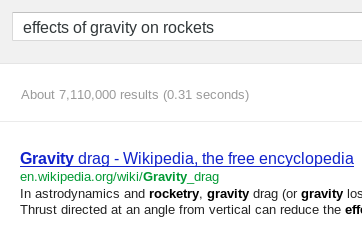
\includegraphics[width=0.80\textwidth]{images/space_rocket_query.png}
\caption{{Google showing over 7M results for ``effects of gravity on rockets"}}
\label{fig:rocket_results}
\end{figure}


Despite their use as general search tools on the World Wide Web, the problem
space that search engines deal with is usually too big for them to find
scientific papers and journals given a set of keywords. Internet search engines
index a huge proportion of irrelevant information compared to useful
information\cite{Berghel1997}, and as a result, even relatively specific
queries such as ``effects of gravity on rockets" yield millions of results (as
shown in Figure \ref{fig:rocket_results}). This shortcoming has already led to
the development of search engines designed specifically to find scientific
papers. 

\subsubsection{Scientific Paper Search Engines}

There are also a number of search and indexing systems that specifically look
for scientific papers as opposed to web pages. One of the most publicised and
well known paper search systems is Google Scholar
(\url{http://scholar.google.com}).  As can be seen in Figure
\ref{fig:scholar_basic}, This is an adaptation of Google's general search
engine (discussed above) to specifically index and search scientific papers.
Google also offers advanced query options specific to Scholar that allow
searching by author, year and for words that occur only in the document title
as shown in figure \ref{fig:scholar_advanced}. Whilst this does deal with the
problem of `information overload' and provides even more fine control over the
information returned from searches,  the user is still required to have a very
good idea of what they are looking for in terms of keywords and/or specific
authors. It is possible that a user would not know what they are looking for
until they've seen it. Even if the user has a set of keywords to search for,
they can only search the title of the paper or the content as a whole. This
means that users who want to find a particular phrase within a CoreSC part of
the paper (e.g. only look for this phrase in the `Result' section of the
paper) are unable to get results at their desired level of detail.

\begin{figure}[!hbt]
        \centering
        \begin{subfigure}[b]{0.50\textwidth}
                \centering
                
\includegraphics[width=\textwidth]{images/googlescholar_front.png}
                \caption{Google Scholar's General front page}
                \label{fig:scholar_basic}
        \end{subfigure}%
        \begin{subfigure}[b]{0.50\textwidth}
                \centering
                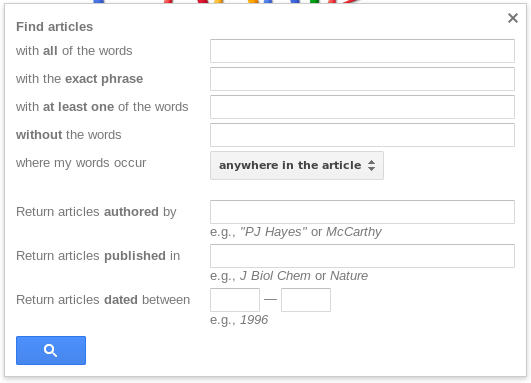
\includegraphics[width=\textwidth]{images/googlescholar_advanced.png}
                \caption{Advanced search features}
                \label{fig:scholar_advanced}
        \end{subfigure}

        \caption{Google Scholar's user interface}
        \label{fig:scholar_interface}
\end{figure}

\subsubsection{Social Citation and Recommendation Engines}
Social citation and recommendation engines also provide a partial solution to
the `information overload' problem.  Services like Goodreads
(\url{http://www.goodreads.com/}) and CiteUlike
(\url{http://www.citeulike.org/}) allow you to register your interest in
specific authors and subjects. This allows the sites to build up a profile of
the sorts of materials that you might be interested in and provide lists of
recommendations as in Figure \ref{fig:social_indexes}.

\begin{figure}[!hbt]
        \centering
        \begin{subfigure}[b]{0.50\textwidth}
                \centering
                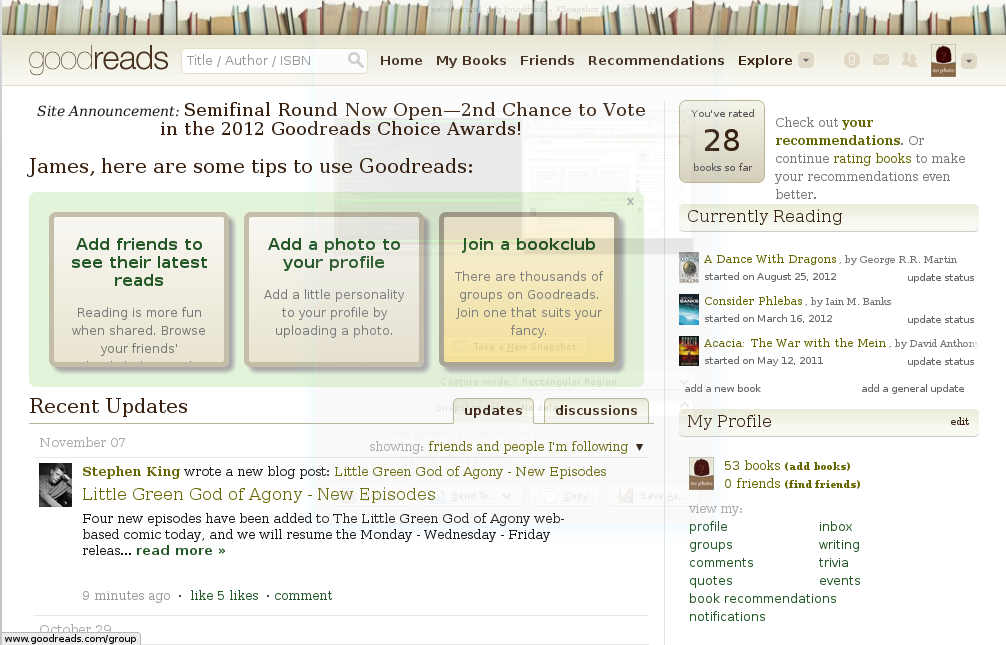
\includegraphics[width=\textwidth]{images/goodreads_index.png}
                \caption{Goodreads user profile page}
                \label{fig:goodreads_index}
        \end{subfigure}%
        \begin{subfigure}[b]{0.50\textwidth}
                \centering
                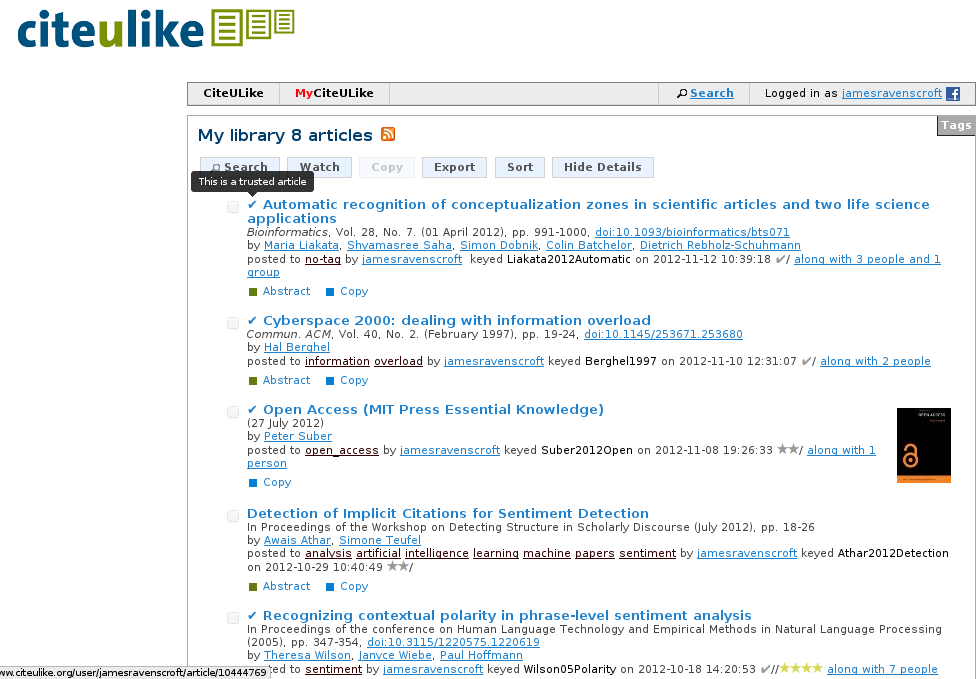
\includegraphics[width=\textwidth]{images/citeulike_index.png}
                \caption{a CiteULike user profile page}
                \label{fig:citeulike_index}
        \end{subfigure}

        \caption{Goodreads and citeulike social recommendation systems}
        \label{fig:social_indexes}
\end{figure}

These systems have the ability to make recommendations to the user without
requiring specific keywords or search terms. They do this by learning the
user's profile and taking into account the preferences of their 'friends' and
their browsing history. However, the above-named systems do not take into
account the content of the paper or book. They only deal with metadata as can
be seen in Figure \ref{fig:social_searches}. This means that important
discriminatory information that could be contained within the actual document
content is overlooked completely. 

\begin{figure}[!hbt]
        \centering
        \begin{subfigure}[b]{0.50\textwidth}
                \centering
                
\includegraphics[width=\textwidth]{images/goodreads_search.png}
                \caption{Goodreads advanced search page}
                \label{fig:goodreads_search}
        \end{subfigure}%
        \begin{subfigure}[b]{0.50\textwidth}
                \centering
                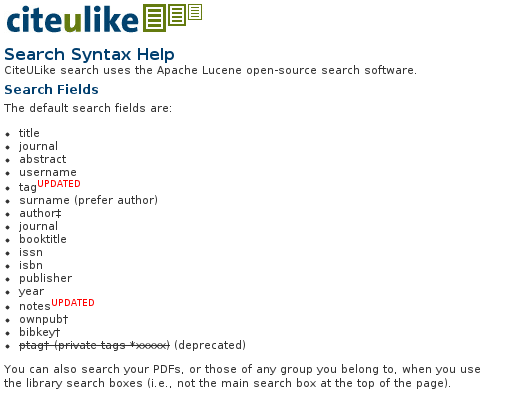
\includegraphics[width=\textwidth]{images/citeulike_search.png}
                \caption{CiteULike advanced search options}
                \label{fig:citeulike_search}
        \end{subfigure}

        \caption{Goodreads and citeulike search only deal with metadata.}
        \label{fig:social_searches}
\end{figure}


\subsection{Methodology}

The language that Partridge will be written in is one of the most fundamental
and important choices to be made. The language choice effects not only the end
performance of the application, but the speed at which the project is developed
and the portability of the end code \cite{britton2008}. It was decided that
Python would be the best language for developing Partridge.

Python is a programming language with a famously shallow learning curve,
readable syntax and dynamic inspection that facilitates rapid prototyping
\cite{bird2009natural}. The language was invented by Guido Van Rossum as a
multi-use, flexible, interpreted scripting language, extensible via compiled C
modules\cite{An93pythonfor}. Developing Partridge in python
would provide a flexible prototyping environment and readable syntax allowing
for investigative work to be carried out quickly and efficiently with minimal
overheads for writing boiler-plate code and debugging. The ability to extend
the language using native code would give Partridge an even greater advantage.
Since NLP techniques can be quite processor intensive and Python is an
interpreted language, and in its very nature, slower than a compiled language,
inefficient sections of Python code could be re-written as C extensions and
compiled into the application. 

Other languages that were considered were Java and C. However, it was decided
that Python's clean syntax and ease of use for prototyping were preferable to
the C and Java style syntax. As stated above, C may still be used in part for
developing Python extensions to improve the overall performance of the
application.

\subsubsection{Web Presentation Frameworks} 

Partridge's web frontend will be used by researchers to wish to query the
system for information on scientific papers. As it is a web tool, Partridge
will be presented as a set of HTML web pages.

For this purpose, the Flask (\url{http://flask.pocoo.org}) library was chosen.
Flask is a python `microframework' for web development. Ronacher (2012) writes
that ``Flask aims to keep the core simple but extensible...[and] won't make any
decisions for you\cite{flask2012}." It uses a simple templating system that can
optionally be swapped out for an equivalent system and does not impose any
limitations or requirements on the layout of the program or the type of
database that is used. Flask also integrates very simply into existing software
using Python annotations\emph{(Ibid)}. 

An alternative approach that was considered was using a separate software
stack such as the Apache web server (\url{http://httpd.apache.org/}) and PHP 
(\url{http://www.php.net}). However, this would involve adding more software to the
project and building an interface between the PHP scripts and Partridge's
python backend. The Django framework (\url{http://www.djangoproject.com/}) for Python was also
considered but it was determined to be overly complicated in terms of
Partridge's requirements.

\subsubsection{Natural Language Libraries} \label{sec:libschoice}.  

It was decided that a pre-existing NLP library should be used to provide
implementations of existing algorithms and techniques for Partridge. For this
purpose the The Natural Language Toolkit (NLTK) was selected. The NLTK is a
simple and intuitive library written for Python. Bird(2009) states that NLTK
was designed ``to provide an intuitive framework along with substantial
building blocks, giving users a practical knowledge of
NLP\cite{bird2009natural}". NLTK provides implementations for sentence
splitting, tagging (the process of analysing sentences and classifying words as
verbs, nouns etc.), and information retrieval from text \emph{(Ibid)}. NLTK
also provides implementations of classifiers and a framework for extracting
features to be used for classification from text. There is also a free book
that accompanies the project available at \url{http://nltk.org/book/} which
provides a huge amount of information on how to implement many popular NLP
techniques using the library.

Some other libraries were considered\cite{mallet2002}\cite{cunningham2011text}.
However, these were written for Java and Partridge is a python project. They
also require a steeper learning curve than NLTK. 

\subsection{Prototyping/Current Work}

\subsubsection{ Sourcing Scientific Papers}
For Partridge to be a success, it is important to include a large variety of
different scientific papers in its corpus. Therefore, several sources of
scientific papers were explored and considered.

The most convenient and accessible source is the ART corpus that SAPIENTA was
trained with\cite{citeulike:11077287}. This corpus is already stored using the
CoreSC schema and has been pre-annotated. This means that Partridge would not
need to do any conversion or pre-processing on the papers. These scientific
papers are all chemistry papers. Therefore, more papers from other scientific
domains are needed to get a wider variety of topics and make Partridge useful
to as wide an audience as possible. 

The `mega-journals' PLOS ONE \url{http://www.plosone.org/} and arXiv
\url{http://www.arxiv.org/} were suggested as sources for more open access
articles that could be added to Partridge. Both of these sites were found to
contain large volumes of open access papers. However, most of these papers were
published as PDF files which meant that some conversion would be required to
make them compatible with Partridge.

\subsubsection{PDF Conversion}
Most scientific papers available on the internet are formatted as PDF
documents. However, Partridge uses and stores documents that use the CoreSC
schema by Soldatova and Liakata\cite{liakata2008guidelines}. Therefore some
spike work was carried out to determine the feasibility of converting papers
published as PDF documents into XML documents. Townsendi et al(2009) liken converting
PDF to XML to ``converting hamburgers into cows," they go on to explain that
PDF documents do not contain any semantic data and documents lose much of their
explicit structure when they are formatted in this way \cite{Townsend2009}.
Therefore, to convert PDF documents into an NLP-friendly format, some
heuristics must be used to detect the document's structure\cite{pdfminer}.

This was the first big challenge in the project. A prototype script was written
using a Python PDF extraction library called PDFMiner
(\url{http://www.unixuser.org/~euske/python/pdfminer/index.html}).  This
toolkit already contains some heuristics about how to extract text from PDF
documents, grouping together characters that appear very close to each other,
and separating paragraphs and headings when a larger area of whitespace is
detected\cite{pdfminer}. Despite these rules, the library still produced some
extraneous whitespace and newline characters as part of the output. A
subroutine to trim whitespace and newlines was added to the script to resolve
this problem. 

The next stage was to split the text into sentences in preparation for
processing with SAPIENTA. With the assistance of the NLTK library, a sentence
splitting subroutine was implemented. This used a machine learning algorithm
that had been trained to recognise sentence boundaries to split the text. Each
sentence was then added to a CoreSC compatible XML document for processing by
SAPIENTA.

Initially, the PDF conversion subroutine had a very high error rate due to the
variation in the formatting of scientific papers. It was suggested that PDFX
(\url{http://pdfx.cs.man.ac.uk/}), a free service hosted by the University of
Manchester could be used instead of PDFMiner for the initial PDF data
extraction. The main advantage of PDFX over the PDFMiner library is that it is a
trained machine learning system that has been trained using a large full-text
selection of scientific articles; PDFMiner uses more general heuristics
designed to process a large selection of different types of PDF document.

PDFX also provides output that already has some metadata, such as title,
author, and abstract, associated with it. PDFMiner did not provide any
metadata, and it was necessary for the script to guess which passage of text
was the abstract after the initial text extraction stage.

With the new PDF extraction method in place, the script ran without the need
to modify either of the whitespace sanitiser or sentence splitter routines. The
process was much more successful and able to produce SAPIENTA-compatible
documents from most of the PDF input files that were provided.

\subsubsection{Pre-processing with SAPIENTA}

With a successful PDF conversion script, the next step was to try and run
SAPIENTA over the converted papers and annotate them, ready for inclusion in
the Partridge corpus.

By default, SAPIENTA is packaged as a web-based tool, written in Java, that
can be downloaded (from \url{http://www.sapientaproject.com/software}) and used
to annotate one paper at a time. Dr Liakata was able to provide information on
two alternative ways of using the system. One method was to submit a remote
procedure call (RPC) to a server running SAPIENTA with a batch of papers and
retrieve the output. The other method was to use an alternative version of the
code that runs locally in a Python environment and could be modified to process
papers as a batch.

A script was written to send un-annotated XML documents to the remote SAPIENTA
server and retrieve a list of annotations. This worked well until the server
stopped replying to requests. This meant that no further conversions could be
carried out until the server was repaired and raised concerns about how the
remote servers might cope with a large number of automated requests from a
full version of Partridge.

The Python version of SAPIENTA was then downloaded and a test executed.
Unfortunately there were several data files missing from the package that had
to be acquired from Dr Liakata. 

SAPIENTA for Python also relies upon a package called CRFSuite which implements
Conditional Random Fields, a method for segmenting and labelling sequence
data\cite{CRFsuite}. This library did not compile properly on the test
environment and its creator had to be contacted via a mailing list (See
Appendix \ref{sec:crfemail}. After a few days, the owner responded and the
library was compiled successfully.  

Once all the data files and libraries were successfully in place, the Python
version of SAPIENTA was used to process some of the papers converted from PDF.
This was a great success and the annotations provided by SAPIENTA seemed to be
accurate. 

\subsubsection{Interface Design}

To help in visualising how the final web frontend will appear, some diagrams of
the user interface have been drawn. You can see these diagrams in Appendix
\ref{sec:ui_designs}. 

\subsubsection{System Processes}

To visualise how some of the system processes will work and how they should be
programmed, some flow diagrams have been produced and attached in Appendix
\ref{sec:system_diagrams}

\section{Planning}

\subsection{Development Methodology}

\subsubsection{Existing Methodologies}
Selecting a suitable development methodology for building Partridge is another
very important choice for the project.

Under the traditional `Waterfall' Software Development model, Requirements
Gathering, Analysis, Program Design, Coding, Testing and Operations were all
defined as formal phases in the development cycle. There is little flexibility
other than moving back up the waterfall to rectify mistakes after
testing\cite{Royce:1987:MDL:41765.41801}. This model was very focused on
paperwork and bureaucracy, trying to maintain a paper trail and manage risk
through accountability \emph{(Ibed)}. This approach to software development is
very heavyweight and slow and often produced software that did not match the
users' needs as a result \cite{Boehm1988}.

As an alternative to the heavyweight Waterfall approach, Beck et al came up
with the principle of the Agile Manifesto, favouring a lightweight, responsive
development model over the heavyweight slow waterfall
system\cite{beck2001agile}. Many of Beck's ideas focus around working in a team
of developers and prioriting communication between team members \emph{(Ibid)}.
This is most prominent in the Extreme Programming (XP) method of software
development. Since Partridge is an individual project, XP is not really
applicable. However, some concepts like rapid prototyping/spike work and
iterative release cycles will be used as part of the Partridge development
methodology.

\subsubsection{ Partridge's Development Methodology}

Partridge is an individual project but does involve discussions with
supervisors. The customers have been identified as the end-users of the system.
Therefore, a customised methodology has been adopted. Firstly, all design and
planning documentation have been written up and placed on a wiki which is
accessible and modifiable by the author and both supervisors. This creates a
paper trail for all tasks and also allows collaboration between involved
parties through the Internet. A full printout of the wiki is available in
Appendix \ref{sec:wiki}. 

Weekly meetings are held with both supervisors. The notes from the preceeding
week are analysed and each task discussed in depth. New tasks are then noted
down along with any observations that should be documented. These new notes are
uploaded to the wiki the following day or earlier. Each party present at the
meeting adds their own observations to the notes page. This page is then
reviewed at the next meeting. As seen in Appendix \ref{sec:wiki}, this practice
has already been running for several weeks and has so far proven to be highly
effective.

Partridge will adopt an Agile approach to release cycles, producing a working
software package at iterations of one month.  Each iteration, the software will
include more of the desired functionality discussed above and in the wiki.
GitHub's issue manager program is being used to track tasks and bugfixes and
plan which tasks will be carried out in which iteration. Tasks that are created
in a full iteration (where no development time is left) will be added to a
backlog and integrated in the next iteration with enough development time to
contain it. Tasks are also assigned a priority, higher priority issues being
tackled before low priority ones.

Partridge's testing strategy consists of multiple unit tests that are run at
integration of new code into the codebase. As soon as the first release is
built, Partridge will be made available for use by the public and users
encouraged to test the system and submit any bugs via the GitHub issue manager.
It is hoped that colleagues at Aberystwyth University and Dr. Liakata's
colleages at the EBI will try to use the system one it becomes available.

\subsubsection{ Work Timeline }

The tasks involved in Partridge have been carefully calculated and prioritised.
They were then added to the GitHub issue management system and a report
generated listing them in the order that they are expected to be
accomplished. This report can be seen in Appendix \ref{sec:timeline}. 


\subsubsection{ Mid-Project Demonstration Plan}

The mid-project demonstration is scheduled for after iteration two of the
Partridge project. If everything runs to schedule, then at this point it will
be possible to demonstrate keyword search within the project's database and
filter based upon the polarity of the paper's results. For redundancy purposes,
Partridge will be configured to run as a server on multiple computers. Both
this and the final project demonstration will require a room with Internet
access. However, should this be unavailable, then Partridge could be run
locally on the author's laptop.

\subsubsection{ Final Project Demonstration Plan}

The final demonstration of Partridge will be fairly similar to the Mid-Project
demonstration. However, it should include all of the planned classifiers and if
there is extra time on the project, the profiling/recommendation engine will
also be demonstrated. This demonstration will use the same redundancy
precautions as the Mid-project demonstration above, and will also need a room
with the internet if available.


%include document appendix

\appendix
\section{User Interface Designs}
\label{sec:ui_designs}

\subsection{ Partridge Query Interface}


Figure \ref{fig:ui_mockup} shows the user interface that will be utilised to
search and query Partridge's corpus. 

The query form shows two main sections: Filters and Keywords. 

Filters can be used to show a large set of papers where the user is unsure of
what to search for. Users will be able to look for papers by type and topic as
discussed above. The paper result filter has not been included in this diagram.
However, it is expected that a drop down menu for result type would be included
in the filters section of the form.

Keywords allows the user to look for a set of keywords that is specifically
within a CoreSC concept for a paper. For example, the reader may want to find
experiments that use a server farm to do lots of calculations. Therefore, they
would enter ``Server Farm" as their keywords and chose ``Method" from the paper
section. The user then adds this to the set of keyword queries in the table
below the text field with the add button.

Once a user has configured both filters and keywords to their preferences, they
click the search form to run the search itself.

Other notable features on this mockup include a list of most recent searches.
This helps the user to understand how to use Partridge and gives them some
suggestions for what they might search for. Similar listings are provided for
the most popular papers in the Partridge database and the most recent papers
added to the system.

\begin{figure}[!ht]
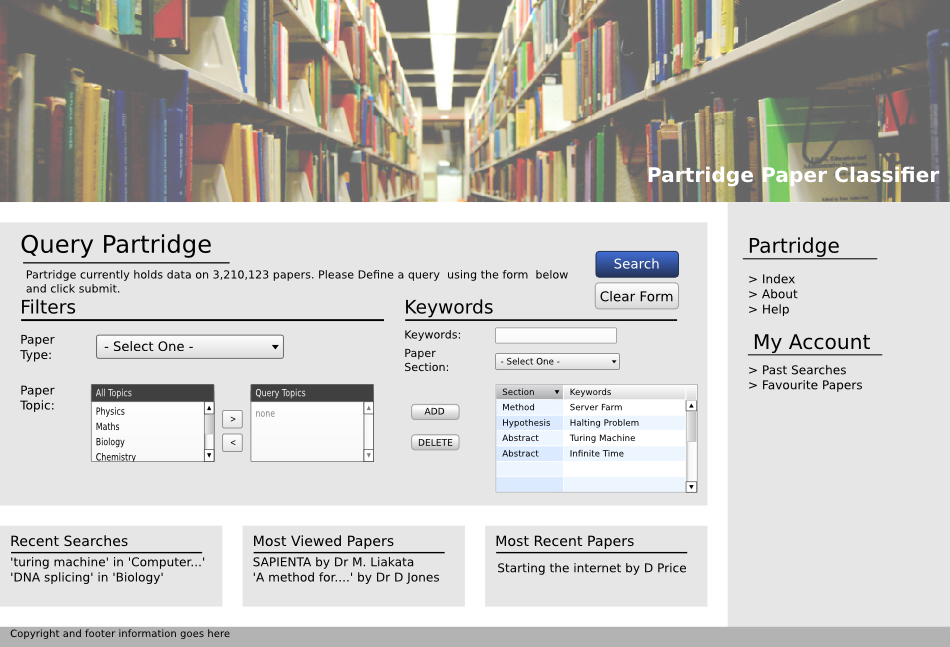
\includegraphics[width=\textwidth]{images/mockup_1.png}
\caption{User interface design for querying Partridge}
\label{fig:ui_mockup}
\end{figure}


\section{System Process Diagrams}
\label{sec:system_diagrams}

This section documents the system process diagrams that have been produced. The
first completed diagram shows how a paper will be added to Partridge and the
actions that will be carried out upon it.

\subsection{Adding a Paper to Partridge}

\begin{figure}[!ht]
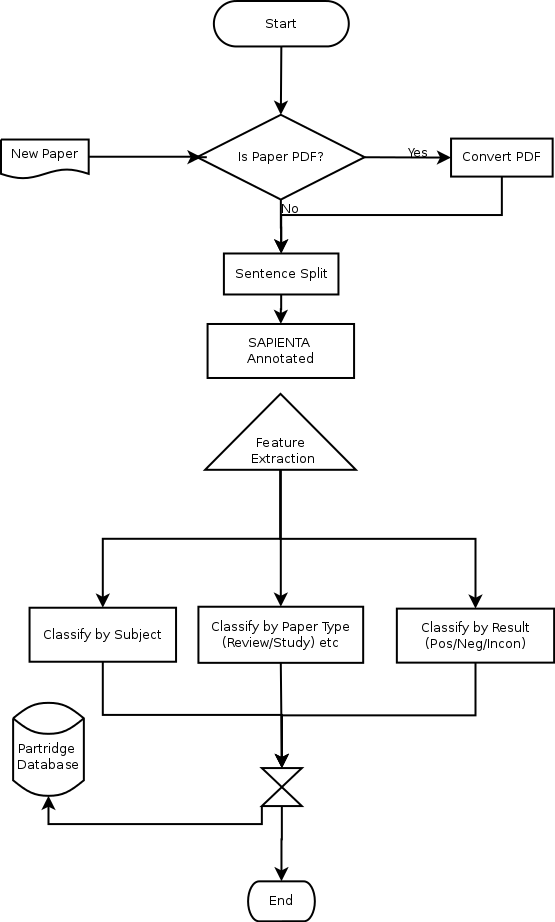
\includegraphics[width=0.75\textwidth]{images/PaperAddedProcess.png}
\caption{The process of adding a new paper to Partridge}
\end{figure}

The system starts off by converting the document to XML from PDF if necessary
through the use of the PDFX tool provided by Manchester University. A sentence
splitting tool is then used to parse the resulting document and separate the
sentences.

Once the sentences have been split, Maria's SAPIENTA tool is used to annotate
each sentence to determine which of the core scientific concepts it covers.
This information is stored back in the XML file with the document.

After this, feature extraction is carried out upon the document to find useful
features for the following classification tasks:

\begin{enumerate}
\item Paper topic/subject -i.e. is the paper a biology paper or a computer science paper?
\item Type of paper - i.e. is the paper a case study, an experiment or a literature review?
\item Paper result - i.e. did the paper have a positive, negative or inconclusive result?
\end{enumerate}

These classifiers are then run (they could potentially be run in parallel if
processing power is available) to determine the paper's class for each
classifier respectively. The data gathered along with any paper metadata
captured such as title, author, date, institute etc are then stored in the
database.


\section{Email for CRFSuite}
\label{sec:crfemail}
\begin{verbatim}
Hi All,

I'm trying to build CRFSuite's python extension 
(http://www.chokkan.org/software/crfsuite/) on an Arch Linux 64-bit 
environment using Swig 2.0.8 (PCRE enabled).

When I run SWIG, I get the following output:

<<OUTPUT OMITTED FOR BREVITY>>

Full output available at http://sourceforge.net/mailarchive/message.php?msg_id=30024209

As far as I can see, all of these problems stem from this declaration in 
the SWIG input file (http://pastebin.com/9JipJ1C1):
%template(ItemSequence) std::vector<CRFSuite::Item>;

I've had a look around on google and on this mailing list and the only 
other "cannot copy typemap" errors I've encountered have been where 
people have excluded the std namespace in favour of a 'using' statement. 
As you can see, this example uses absolute class names so that isn't the 
issue here. I haven't had any luck contacting the software maintainer 
for CRFSuite yet either.

As you might expect, if I continue to compile the extension without 
heeding these errors, when I try to make use of the ItemSequence object 
I get the following python error:
TypeError: in method 'ItemSequence_append', argument 2 of type 
'std::vector< CRFSuite::Item >::value_type const &'

I'm going to keep trying to sort this out and if I find the solution 
independantly, I'll make sure to post a follow-up email. However, if 
anyone else has any ideas about what might be happening here, please let 
me know.

Thanks,

James Ravenscroft
AI & Robotics Undergraduate
Aberystwyth University
\end{verbatim}


\section{Project Timeline}
\label{sec:timeline}

This table shows the projected timeline for the Partridge project. These
calculations were carried out under the assumption of 2 full days of work per
week on the project and one iteration equating to one month (28 days). There
will be 7 iterations in total and after each, a new version of Partridge will
be made available (except for iteration zero which is a research only
iteration).


\begin{figure}[htp] 
 \vspace{ -1cm }
 \centering{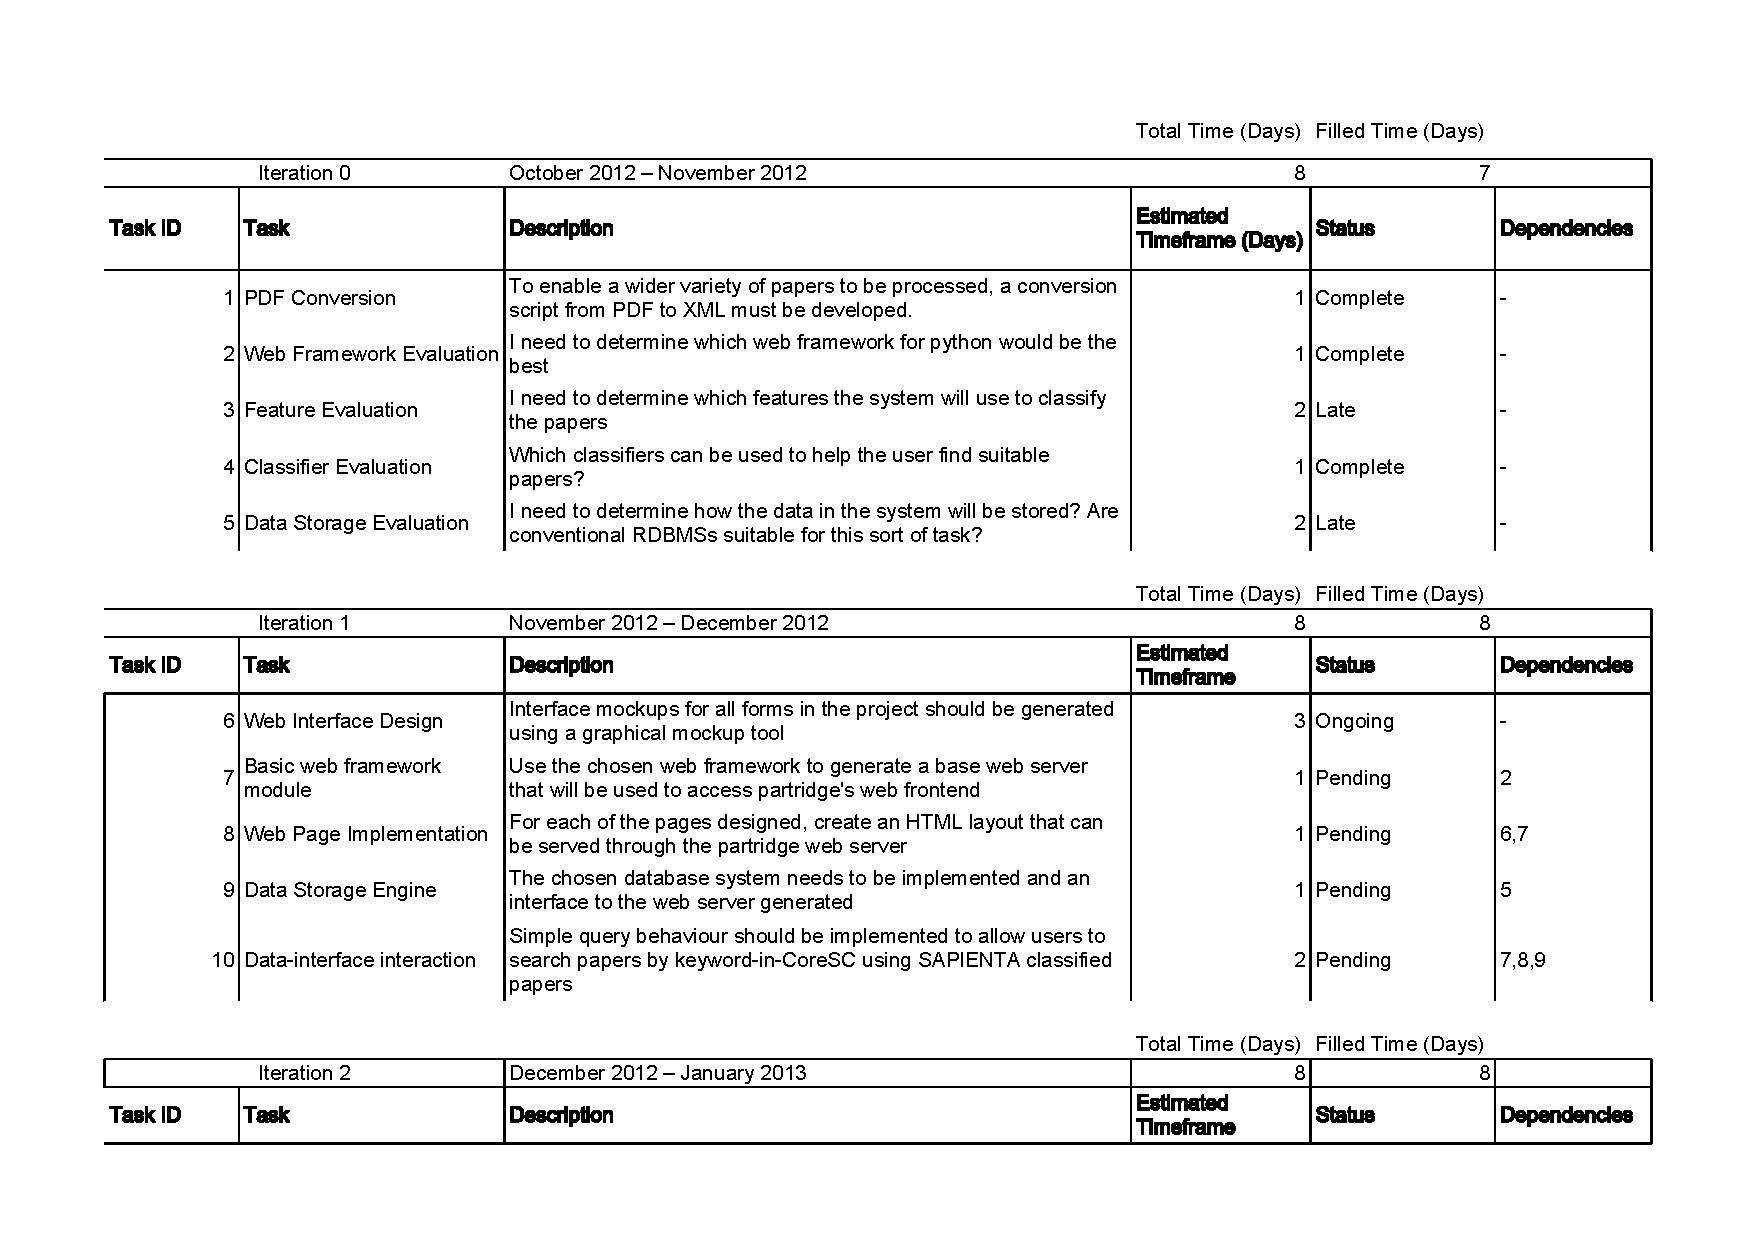
\includegraphics[scale=0.60,page=1]{../timeline.pdf}}
  
\end{figure}

\begin{figure}[!htp] 
 \centering{\includegraphics[scale=0.60,page=2]{../timeline.pdf}}
 \vspace{-2cm}
\centering{\includegraphics[scale=0.60,page=3]{../timeline.pdf}}
\end{figure}

\pagebreak
\section{Project Wiki}
\label{sec:wiki}

All pages from the Wiki are shown below with the exceptions of those pages
which have already been mostly featured in the document (UI Mockups and
Progress Diagrams and the project timetable are not shown in this section).

\subsection{ Notes 03/10/2012 }
\subsection{Meeting Notes from 03/10/2012}

\subsubsection{General topics}

\begin{itemize}
\item
  Talked about using research papers instead of books :-
\item
  copyright issues - mainly resolved because of Gutenburg project
\item
  processing issues - too much information to process quickly and
  realistically
\item
  Maria has some software for identifying sections in papers - could be
  used to help locate specific features
\item
  There are quite a few sources for papers that could be used for the
  project:
\item
  http://arxiv.org/
\item
  http://plosone.org/
\item
  Maria's papers are in XML format
\item
  Formatting may or may not be an issue - PDFs are a nightmare to parse
\end{itemize}

\subsubsection{Things to consider}

\begin{itemize}
\item
  What sort of recommendations for different sources might there be and
  how would these recommendations be extracted?
\item
  Feature engineering - what sorts of features might there be to pick
  out in the papers?
\item
  I need to have a read through the sentiment analysis paper that Maria
  has been working on
\item
  I need to have a play with the software for identifying sections in
  papers.
\end{itemize}

\subsubsection{Misc concerns}

\begin{itemize}
\item
  Decided that our weekly meeting should be Wednesdays at 3pm
\item
  Investigate setting up source control and a wiki (that's been done as
  you can tell)
\end{itemize}


\subsection{ Notes 10/10/2012 }
\subsection{Meeting Summary 10/10/2012}

\subsubsection{From Maria's notes}

\begin{itemize}
\item
  James has gone through papers and thinks would be more doable to work
  with papers than Books
\item
  James has found the XML format of PlosOne and ART/CoreSC corpus
\item
  Domain needs to be determined
\item
  Maria to send paper on sentiment analysis of citations
\end{itemize}

\subsubsection{Current features and recommendations}

\begin{itemize}
\item
  Analysis of results section - positive or negative result
\item
  Potentially look at writing styles of authors using syntactic analysis
\item
  Isolating terms within sections of papers (i.e.~find me papers where
  methodology x was used)
\item
  finer grain analysis of CoreSC categories
\item
  nltk python toolkit. What other toolkits? Would jerboa be any good?
\item
  common features for sentiment analysis
\end{itemize}

\subsubsection{Basic system design}

I have started a basic system design although it is very basic at the
moment. [Image Omitted]

\subsubsection{Background - Similar Systems and how they work}

\begin{itemize}
\item
  Google Scholar
\item
  Mendeley
\item
  Citeulike
\item
  Tweeting or `liking' on facebook.
\end{itemize}

\subsubsection{Reading}

\begin{itemize}
\item
  TF-IDF
\item
  Take a brief look at journal of negative results
\item
  `Bigrams + trigrams' and syntactic pattern finding
\item
  Common features used in NLP
\item
  Sentiment analysis of citations in papers
\item
  `Bag of words'
\end{itemize}

\subsubsection{Coding/practical research}

\begin{itemize}
\item
  Play some more with SAPIENTA
\item
  Implement a (La)TeX to SciXML or pubmed command-line tool.
\end{itemize}


\subsection{ Notes 19/10/2012 }
\subsection{Notes from Meeting 18/10/2012}

\subsubsection{General Comments}

\begin{itemize}
\item
  I need to decide on a domain for the project. It may be that papers on
  a varied selection of topics would be a good start
\item
  Decided on an agile development cycle with a basic program that is
  improved in `iterations'.
\item
  As part of testing the software, it may be possible to get other final
  year students to trial the engine and use it to make recommendations
  for their reading.
\item
  I need to investigate ways of analysing papers for syntactic patterns.
  This may be indicative of:

  \begin{itemize}
  \item
    Different authors' writing styles
  \item
    Different types of paper -i.e.~psychology vs physics
  \end{itemize}
\end{itemize}

\subsubsection{TODO}

\begin{itemize}
\item
  Revisit PDF to XML conversion as conversion from PDF would make life a
  lot easier
\item
  Maria mentioned that she may have access to an HTML to XML program
  which would be good to look at.
\item
  Check out python Jerboa to see if it would be useful for the project.
\end{itemize}


\subsection{ Notes 24/10/2012 }
\subsection{Notes from meeting 24/10/2012}

Amanda was not present for this meeting.

\subsection{Discussed}

\begin{itemize}
\item
  We discussed the PDF conversion routine and decided that whilst
  important, it is crucial not to get too caught up in this.
\item
  Maria is going to send me a link to an existing PDF to XML converter
  that might provide the functionality with some tweaking - or at least
  help
\item
  We discussed the Python version of Sapienta which currently supports
  SciXML and simplified versions thereof.
\item
  Maria needs to send me a couple of data files for this to work
  properly.
\item
  Confirmed that Jerboa is a Java library (I was confused because I was
  expecting a python toolkit) and need to look at it properly now.
\item
  Discussed the actual functionality of the system and came up with a
  brief system outline, around which I can plan.
\end{itemize}

\subsection{TODO}

\begin{itemize}
\item
  Now that we know what the system is going to do (See System Outline), I need to look at features that
  will allow us to:
\item
  Pre-classify documents based on their topic, type, result etc
\item
  Determine document similarity based on user preference from their
  tagging etc. (I can make use of the ``Features in sentiment analysis''
  paper for this)
\item
  Run more tests on the PDF parser and potentially look at another
  solution if this takes up too much time.
\item
  Have a go with Python SAPIENTA once the data models are present
\end{itemize}


\subsection{ Notes 31/10/2012 }
\subsection{James' Meeting Notes}

\subsubsection{To Think about}

\begin{itemize}
\item
  Discussed imminent deadline for project progress report - 19/11/2012
\item
  Decided that having a report finished by 14/11/2012 would be a good
  report to give Amanda and Maria a chance to check over the report
  before handin.
\item
  Maria explained that it is possible to send a batch of papers to
  Sapienta rather than one at a time. She is going to provide
  information on how this can be achieved at some point during the week.
\item
  I should describe my working processes and why they are helpful.
\end{itemize}

\subsubsection{Todo}

\begin{itemize}
\item
  We discussed the merits of using the pdfx converter instead of my
  script - might have plug-and-play compatibility with Sapienta for a
  start - need to verify this.
\item
  I need to send my error message the CRFSuite compilation to Maria so
  that she can contact the maintainer.
\item
  I need to expand on the system outline providing more specific goals
  and timeframes - this will become my development plan.
\item
  I need to look at textpresso and see if it will help me with my
  comparison/evaluation
\end{itemize}


\subsection{ Notes 07/11/2012 }
\subsection{Notes from 7/11/2012}

\subsubsection{Discussed}

\begin{itemize}
\item
  What I'll need to have for my demo:

  \begin{itemize}
  \item
    Simple web interface
  \item
    Few basic classifiers - probably result of paper positive/negative
    and maybe paper type - proportions of coreSC concepts.
  \item
    Could show off PDF to XML converter script
  \end{itemize}
\end{itemize}

\subsubsection{To Consider}

\begin{itemize}
\item
  Is the disparity between bio paper CoreSC classification and other
  sorts of paper to do with Sapienta's model or does it demonstrate a
  feature - different subjects may have different proportions of each
  concept.
\item
  If I'm using distribution of concepts as an aggregate feature, I need
  to make sure the system does not fall over if a concept is missing.
\item
  Front end interface:
\item
  Need to find a new word for `section' Scientific Concept may be a bit
  too `scary', is there a better term for this?
\item
  If I allow users to upload papers, they must sign a digital disclaimer
  to say that they have the right to do so
\item
  There should be a ``report copyrighted material'' system
\end{itemize}

\subsubsection{To Do}

\begin{itemize}
\item
  Biggest task this week: Progress Report.

  \begin{itemize}
  \item
    Draft due 14/11/2012 for discussion on 15/11/2012
  \item
    Final deadline 19/11/2012
  \item
    Could provide wiki content as an appendix to the report
  \item
    Come up with a project timeline - actually consider dates
  \item
    Start with the web interface and work upwards.
  \end{itemize}
\item
  Send Maria the missing header file from crfsuite
\item
  Link system outline from wiki index
\item
  Maria said she'd look for a topic detection paper for me to peruse
\item
  I need to have another look at relevant features - struggling with
  this
\item
  Make a wiki list of features that could be used for classification
\end{itemize}




\pagebreak
\bibliographystyle{IEEEannot}
\bibliography{report}


\end{document}
